\section{Einleitung} % (fold)
\label{sec:einleitung}

Der Reinst-Germanium-Detektor ist ein Messinstrument in der $\gamma$-Spektroskopie.
Der Detektor besitzt im Vergleich zu anderen Detektoren ein hohes Energieauflösungsvermögen und in diesem Versuch werden die $\gamma$-Spektren verschiedener Proben untersucht.

\section{Theorie} % (fold)
\label{sec:theorie}

\subsection{Wechselwirkung von $\gamma$-Strahlung mit Materie} % (fold)
\label{sub:wechselwirkung_von_gamma_strahlung_mit_materie}

Tritt ein $\gamma$-Quant mit Materie in Wechselwirkung, sind für die $\gamma$-Spektroskopie besonders der Photoeffekt, der Compton-Effekt und die Paarbildung von Interesse.
Diese Effekte führen zu einem vom Wirkungsquerschnitt $\sigma$ abhängigen Intensitätsverlust des $\gamma$-Strahls.
Die Intensität kann mithilfe der Gleichung

\begin{equation}
	N(D) = N_\text{0} \left(1-\exp\left(- n \sigma D\right)\right)
\end{equation}

beschrieben werden.
Dabei ist $D$ die Absorberschichtdicke, $N_\text{0}$ die ursprüngliche Strahlintensität und $n$ die Teilchendichte des Absorbers.\\

Die mittlere Reichweite $\bar{x}$ der $\gamma$-Quanten ist durch den reziproken Wert des Extinktionskoeffizenten gegeben.
Unter der Annahme von isolierten Elektronen der Absorberatome ist dieser durch

\begin{equation}
	\mu = n \sigma = \frac{z N_\text{L} \rho}{A} \sigma
\end{equation}

gegeben.
$A$ entspricht dem Atomgewicht, $\rho$ der Dichte, $z$ der Kernladungszahl und $N_\text{L}$ der Loschmidtschen Zahl.\\

Beim Photoeffekt muss die Energie des $\gamma$-Quants $E_\gamma$ größer sein als die Bindungsenergie $E_\text{B}$ der Elektronen.
Dabei gibt der $\gamma$-Quant seine gesamte Energie an das Elektron ab, sodass dieses die Energiedifferenz als kinetische Energie erhält.
Die entstandenen Elektronenlöcher werden unter Aussendung charakteristischer Röntgenstrahler von einem Elektron einer höheren Schale aufgefüllt.
Der Wirkungsquerschnitt des Photoeffekts ist durch

\begin{equation}
	\sigma_\text{ph} \propto z^\alpha E^\delta \label{photo_quer}
\end{equation}

gegeben mit 4 < $\alpha$ < 5 und $\delta \approx$ -3,5.\\

\begin{figure}
	\centering
	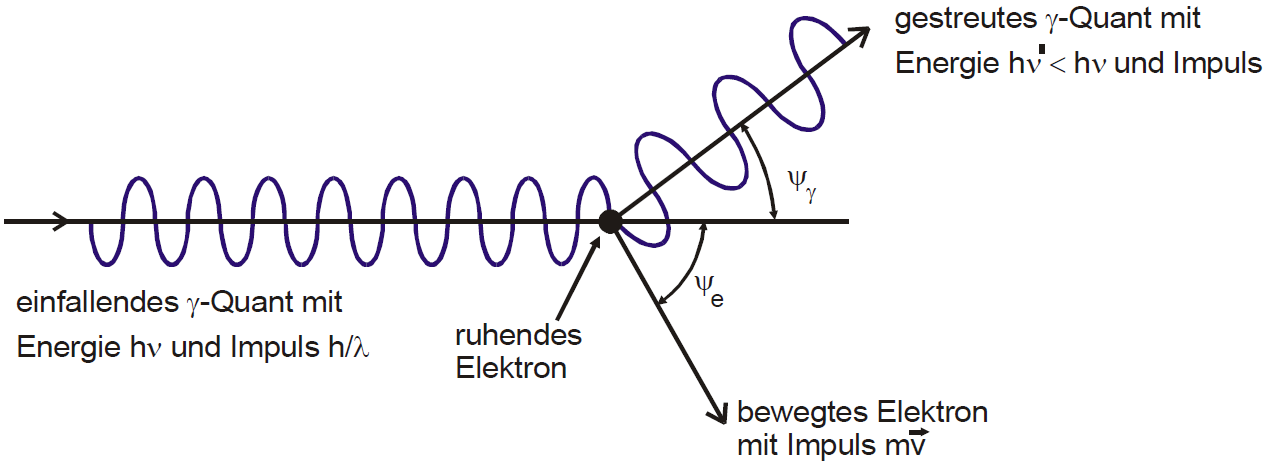
\includegraphics[width = 0.5\textwidth]{pic/compton.png}
	\caption{Schematische Darstellung der Compton-Streuung \cite{anleitung}.}
	\label{compton}
\end{figure}

Der Compton-Effekt kann als inelastische Streuung des $\gamma$-Quants an einem praktisch ruhenden Elektron verstanden werden.
Mit

\begin{equation}
	\epsilon = \frac{E_\gamma}{m_\text{0} c^2}
\end{equation}
ergibt sich nach Abbildung \ref{compton} für die Energie des gestoßenen Elektrons

\begin{equation}
	E_\text{el} = E_\gamma - E_{\gamma'} = E_\gamma \frac{\epsilon (1-\cos{\Psi_\gamma})}{1 + \epsilon (1-\cos{\Psi_\gamma})} . 
\end{equation}

Somit ist der maximale Energieübertrag durch 

\begin{equation}
	E_\text{el,max} = E_\gamma \frac{2\epsilon}{1+2\epsilon} < E_\gamma
\end{equation}

gegeben.
Somit ist der Compton-Effekt eine unerwünschte Erscheinung, da nur ein sich verändernder Bruchteil der $\gamma$-Energie detektiert wird.\\

\begin{figure}
	\centering
	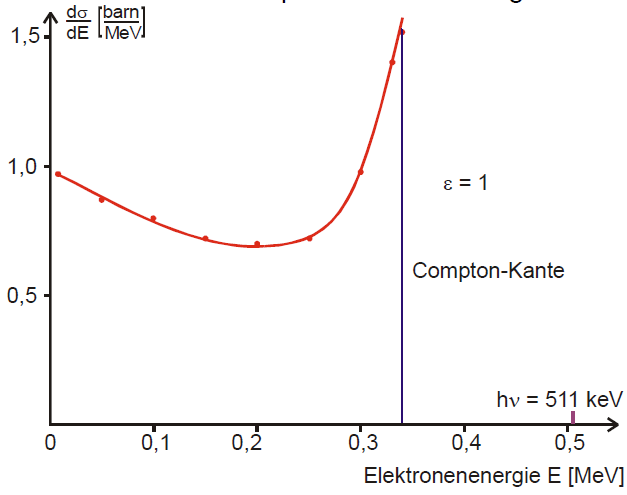
\includegraphics[width = 0.5\textwidth]{pic/compton2.png}
	\caption{Differentieller Wirkungsquerschnitt für die Compton Streuung bei $\epsilon = 1$ \cite{anleitung}.}
	\label{compton2}
\end{figure}
Bei kleinen Energien gilt für den Wirkungsquerschnitt 

\begin{equation}
	\sigma_\text{Co} = \frac{3}{4} \sigma_\text{Th} \left(1 - 2\epsilon + \frac{26}{5} \epsilon^2 + ...\right) .
\end{equation}

Für $\epsilon \rightarrow 0$ gilt

\begin{equation}
	\sigma_\text{Co} = \sigma_\text{Th} = \frac{8}{3} \pi r_\text{el}^2 . 
\end{equation}

Da Detektoren nur die Elektronenenergie detektieren, ist die Energieverteilung der gestoßenen Elektronen wichtig.
Diese ist durch den differentiellen Wikrungsquerschnitt $\frac{\text{d}\sigma}{\text{d}E}$ gegeben.
In Abbildung \ref{compton2} ist eine beispielhafte Kurve dargestellt.\\
\FloatBarrier

Die Paarbildung beschreibt das Entstehen eines Elektronen-Positronen Paares durch die Wechselwirkung eines $\gamma$-Quants mit einem Stoßpartner.
Ist dies ein Atomkern, so muss die Energie des $\gamma$-Quants größer als $2 m_\text{0} c^2$ sein und im Falle eines Elektrons sogar $4 m_\text{0} c^2$.
Die Differenz der Energien wird im gleichen Maße auf das Elektron und das Positron übertragen wodurch sich eine symmetrische Verteilungskurve ergibt.

Für die Grenzfälle des Wirkungsquerschnittes im Falle verschwindender und vollständiger Abschirmung ergiebt sich

\begin{eqnarray}
	\text{Verschwindend: } \sigma_\text{Pa} &=& \alpha r_\text{el}^2 z^2 \left(\frac{28}{9} \ln(2\epsilon) - \frac{218}{27}\right) ,\\
	\text{Vollständig: } \sigma_\text{Pa} &=& \alpha r_\text{el}^2 z^2 \left(\frac{28}{9} \ln(\frac{183}{\sqrt[3]{}}) - \frac{2}{27}\right) .
\end{eqnarray}

Nach der Bildung können das Elektron oder das Positron oder gar beide Teilchen aus dem Detektor austreten.
Zudem kann auch durch Bremsstrahlung ein Energieverlust zustande kommen.
Somit verbreitert sich das Spektrum zu kleineren Energien hin.
\FloatBarrier
\subsection{Der Aufbau und die Wirkungsweise eines Reinst-Germanium-Detektors} % (fold)
\label{sec:der_aufbau_und_die_wirkungsweise_eines_reinst_germanium_detektors}

Der Germaniumdetektor ist ein Halbleiterdetektor und besteht daher aus zwei aneinander angrenzenden Bereichen, welche unterschiedlich dotiert sind.
Durch den Potentialunterschied kommt es zur Ausbildung einer ladungsträgerarmen Zone, welche durch das Anlegen einer äußeren Spannung und eine stark asymmetrische Dotierung vergrößert werden kann.
Die angelegte Spannung sollte jedoch nicht zu hoch gewählt werden, da es ansonsten zu spontaner Bildung von Ladungsträgerpaaren kommt.
Um dem entgegenzuwirken wird der Detektor üblicherweise mit flüssigem Stickstoff gekühlt.

Tritt ein $\gamma$-Quant in die Zone ein, kann es zur Freisetzung eines energiereichen Elektrons kommen, welches wiederum mit anderen Elektronen des Valenzbandes wechselwirkt und seine Energie an diese abgiebt und diese wiederum mit weiteren wechselwirken.
Die erzeugten Elektronen-Loch-Paare können auf Elektroden gespeichert werden und die resultierende Spannung ist proportional zur Energie des eingefallenen $\gamma$-Quants.

Für den Extinktionskoeffizienten in Abhängigkeit der Energie des $\gamma$-Quants ergeben sich für die verschiedenen Wechselwirkungen die in Abbildung \ref{german} dargestellten Kurven.\\

\begin{figure}
	\centering
	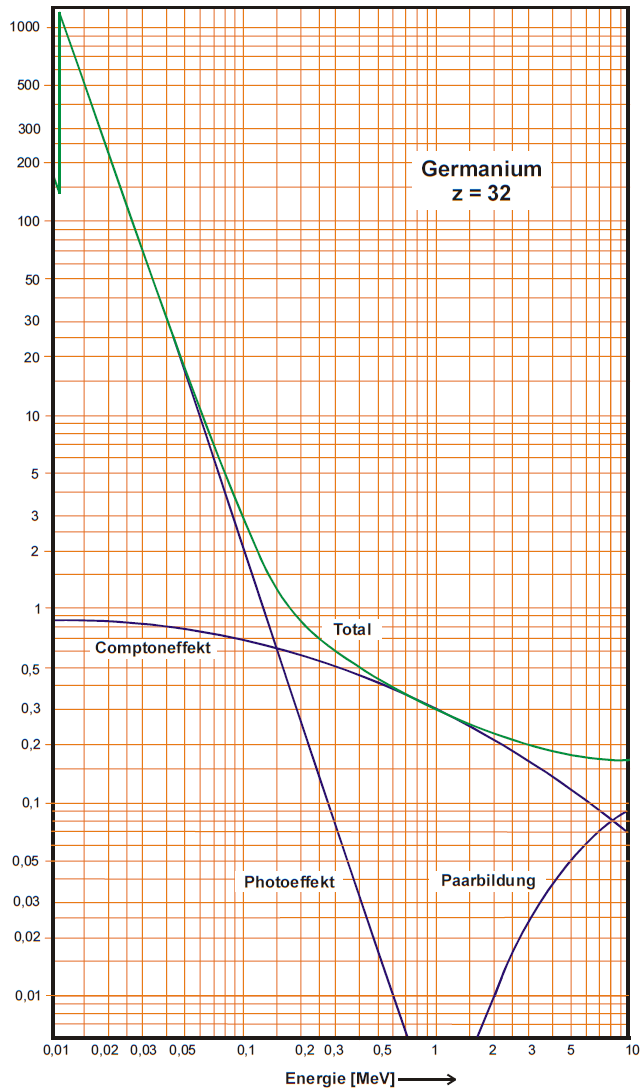
\includegraphics[width = 0.5\textwidth]{pic/german.png}
	\caption{Energieabhängigkeit des Extinktionskoeffizienten $\mu$ für Ge getrennt nach den verschiedenen Wechselwirkungsmechanismen \cite{anleitung}.}
	\label{german}
\end{figure}

Der hier verwendete Detektor ist in Abbildung \ref{detekt} dargestellt.
Um die Oberfläche gut leitend zu machen, ist diese mit Li-Atomen n-dotiert, während das Innere des Zylinders mithilfe von Gold stark p-dotiert worden ist.
Der gesamte Detektor ist zudem von einer Aluminium Schicht umgeben.
Zusammen mit der Li-dotierten Oberfläche führt dies zu einer unteren nachweisgrenze für die $\gamma$-Energie von etwa $\SIrange{40}{50}{\kilo\electronvolt}$, da die $\gamma$-Quanten diese beiden Schichten zunächst durchdringen müssen.

\begin{figure}
	\centering
	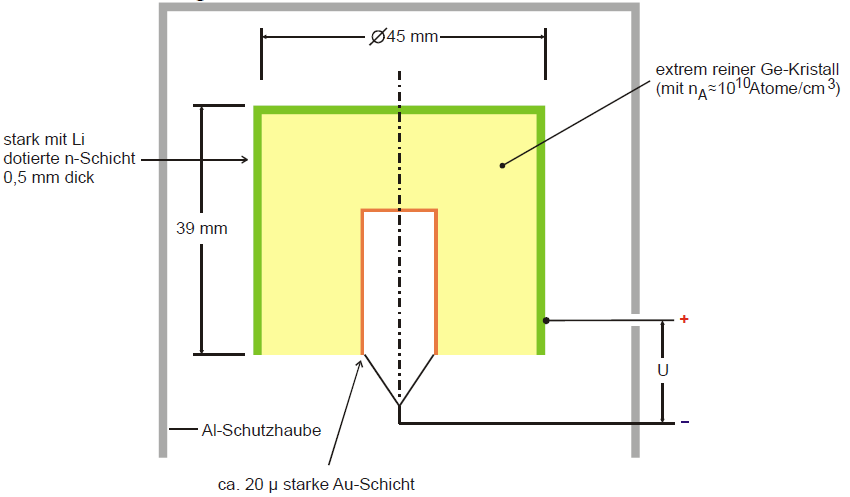
\includegraphics[width = 0.5\textwidth]{pic/detekt.png}
	\caption{Querschnitt durch einen koaxialen Reinst-Ge-Detektor \cite{anleitung}.}
	\label{detekt}
\end{figure}

\FloatBarrier
\subsection{Eigenschaften eines Halbleiter-Detektors} % (fold)
\label{sec:eigenschaften_eines_halbleiter_detektors}

Das energetische Auflösungvermögen des Detektors ist eine wesentliche Kenngröße für die $\gamma$-Spektroskopie.
Diese wird über die Halbwertsbreite $\Delta E_\text{1/2}$ bestimmt, welche angiebt wann sich zwei unterschiedliche Spektrallinien bei einfall monochromatischer $\gamma$-Strahlung noch zuverlässig voneinander trennen lassen.
